


\subsection{Routing}
\subsubsection{Traditionelles Routing}
Routingalgorithmen werden benötigt, um Pfade für den Datenverkehr innerhalb eines Netzwerks zu finden. Beim traditionellen Routing erstellt jeder Router eine Routingtabelle, die Netzwerkadressen und Netzmasken enthält. Anhand dieser Tabelle, bei der diese Adressen auch Geräte zugeordnet sind, können dann Pakete durch das Netzwerk weitergeleitet bzw. geroutet werden. Bei der Suche nach einer geeigneten Route durch das Netzwerk wird klassischerweise ein Longest Prefix Match durchgeführt. Bei einem Treffer wird das Paket im entsprechenden output port weitergeleitet, ansonsten wird der default link genommen. Die Routingtabellen werden durch eine Analyse der vorhandenen Netzwerktopologie aufgestellt. Sollte sich die Topolgie im Betrieb ändern, muss daher auch die Routingtabelle angepasst werden. Routingschemata werden üblicherweise als Graphen dargestellt, wobei die Knoten die Kommunikationsteilnehmer und die Kanten die Leitungen zwischen den Teilnehmern darstellen. Die Kanten enthalten auch Informationen über die Kosten für die Paketübertragung zwischen Knoten. Die Kosten beziehen sich dabei meistens auf die physikalische Länge der Leitung, je länger die Leitung desto höher sind auch die Kosten. Da es bei der Wegfindung zwischen zwei nicht direkt benachbarter Knoten häufig mehrere Alternativen gibt, werden die nötigen Gesamtkosten die zwischen Anfangs- und Zielknoten auftreten, bei der Wahl des Pfades berücksichtigt. Beim traditionellen Routing wird also vorrangig nach den kostengünstigsten Pfaden zwischen Knoten innerhalb eines Netzwerks gesucht.
\\Routing-Algorithmen lassen sich in zwei Klassen aufteilen:
\begin{itemize}
\item Globaler Routing-Algorithmus: Hierbei ist das komplette Netzwerk bereits vor der Berechnung der kostengünstigsten Route bekannt. Es können direkt alle möglichen Pfade zwischen Ausgangs- und Zielknoten und deren Gesamtkosten bestimmt werden.
\item Dezentraler Routing-Algorithmus: Die Knoten haben hierbei nur Informationen über die Knoten und Kanten, welche sich in der Nähe befinden, das komplette Netzwerk ist nicht bekannt. Das Finden eines geeigneten Pfades kann also nur iterativ von Knoten zu Knoten geschehen und nicht bereits im Voraus.  
\end{itemize}
Da das Ziel dieser Arbeit ein semantischer Broadcast ist, bei dem sich die Kommunikationspartner vorher nicht kennen müssen, wird es sich bei dem Algorithmus um einen dezentralen Routing-Algorithmus handeln.
\\Eine weitere wichtige Unterscheidung bei Routing-Algorithmen ist die Frage, ob diese statisch oder dynamisch gestaltet sind:
\begin{itemize}
	\item Statische Routing-Algorithmen werden benutzt, wenn sich die Kanten zwischen den Knoten nur selten ändert. Die Netzwerktopologie bleibt also konstant.
	\item Bei Dynamischen Routing-Algorithmen werden bei sich häufig ändernden Netzwerktopologien eingesetzt. Sie müssen anders als die statischen Algorithmen den stetigen Wechsel von Knoten, Kanten und Kosten beachten.
\end{itemize}
Das Ergebnis dieser Arbeit wird in einer mobilen Applikation eingebunden werden und soll von natürlichen Personen per Smartphone bedient werden können. Der Routing-Algorithmus muss also zwingend dynamisch sein, da Menschen mit ihren Smartphones anders als andere Netzwerkgeräte konstant in Bewegung sind. Da bei einem Broadcast unabhängig von den Kosten die Nachricht zunächst an alle Personen geschickt werden wird, handelt es sich zusammengefasst um einen dezentralen, dynamischen und lastinsensitiven Routing-Algorithmus. 
\subsubsection{Inhaltsbasiertes Routing}
Beim inhaltsbasierten Routing wird für die Bestimmung des Pfads nicht die Zieladresse des Pakets ausgewertet, sondern die semantische Beschreibung des Paketinhalts. Jedes Paket verfügt daher über eine Inhaltsbeschreibung, wobei dann alleine von dieser Beschreibung abhängig ist, an welchen Knoten die Nachricht weitergeleitet wird. Eine wichtige Voraussetzung für diese Art von Routing ist ein Peer-To-Peer (P2P) Netzwerk, da die Pakete stets nur von Punkt zu Punkt gesendet werden. Die Peers müssen ebenfalls ein Interesse formulieren können, anhand dessen bestimmt werden kann, ob ein Paket für sie relevant ist. Dies geschieht meist über themengesteuerte Abonnements. Peers können über diese Abonnements ihr Interesse an einer bestimmten Gruppe von Paketen bekunden. Es gibt zwei unterschiedliche Arten, diese Abonnements innerhalb eines Netzwerks zu verwalten:
\begin{itemize}
	\item Die Abonnements werden ausschließlich vom Peer selbst für die Auswertung herangezogen, andere Peers können diese nicht berücksichtigen. Die Pakete müssen nach der Auswertung durch den Peer dann an alle verfügbaren Peers in der Nähe weitergeleitet werden, da deren Abonnements unbekannt sind. 
	\item Die Peers teilen Ihre Abonnements den anderen Teilnehmern im Netzwerk mit. Dadurch können die Pakete nun gezielt nur an die Peers weitergeleitet werden, die sich für das Paket auch interessieren.
\end{itemize}
Beide Lösungsansätze haben Vor- und Nachteile. So hat der zweite Ansatz den Vorteil, dass nicht bei jedem Peer eine semantische Prüfung der Paketbeschreibung erfolgen muss, da diese Filterung bereits beim sendenden Peer vorgenommen worden ist. Der entscheidende Nachteil dieses Ansatzes ist jedoch, dass sämtliche Modifikationen an bestehenden Abonnements jedem Peer im Netzwerk mitgeteilt werden muss. Bei der App dieser Arbeit ist davon auszugehen, dass Benutzer ihre Abonnements (bzw. Profile) häufig editieren, was zu einer Flut an Benachrichtigungen zu anderen Peers führen könnte. Es ist bei dem Ad-Hoc Broadcast auch nicht realistisch davon auszugehen, dass jeder Peer die Abonnements der anderen Peers kennt, bevor der Benutzer eine Nachricht versendet. Da das Protokoll vorrangig von leistungsstarken Smartphones und nicht von eher leistungsschwachen Kleinstgeräten benutzt werden soll, ist der durch die wiederholte semantische Auswertung der Paketbeschreibung nötige Aufwand vernachlässigbar. In dieser Arbeit wird daher der erstgenannte Lösungsansatz verfolgt. 
\subsubsection{Broadcast-Routing}
Wenn ein Paket an alle interessierten Peers innerhalb eines Netzwerks verschickt werden soll, wird ein Broadcast-Routing benötigt, da das bisher beschriebene Unicast-Routing nur die Wegfindung zwischen zwei Knoten realisiert. Häufig sind für einen Knoten nicht alle anderen Knoten des Netzwerks direkt erreichbar, es werden also Zwischenstationen benötigt welche die Nachricht weiterleiten. Anders als beim Unicast-Routing ist die Anzahl der Pfade also variabel, je nachdem wie viele Knoten das Paket an ihre Nachbarknoten weiterleiten. Wenn ein Knoten eine Nachricht an alle Nachbarknoten schickt und diese sie wiederum an ihre Nachbarknoten schicken, wird dieser Ansatz \textit{flooding} genannt. \textit{Flooding} kann bei unbedachtem Einsatz zu Schleifen führen. Hierbei erhält und versendet ein Knoten wiederholt Nachrichten, die er bereits verwertet hat. Dieser endlose Ping-Pong-Effekt zwischen den Nachbarknoten führt dann zum sogenannten \textit{Broadcast storm}, der das gesamte Netzwerk unbrauchbar macht. \textit{Flooding} muss also zwingend kontrolliert werden, die Knoten müssen unabhängig von der semantischen Überprüfung der Nachrichten prüfen können, ob sie eine eingehende Nachricht bereits verwertet haben. In der Praxis wird meistens einer der folgenden drei Lösungsansätze für dieses Problem gewählt:
\begin{itemize}
	\item Beim sequenznummerkontrollierten \textit{Flooding} schickt jeder Knoten seine Adresse und eine Broadcast-Sequenznummer an seine Nachbarknoten. Dadurch kann jeder Knoten eine Tabelle anlegen, die bereits empfangene Pakete den Nachbarknoten zuordnet. Bei eingehenden Paketen wird nun vorher überprüft, ob dieses Paket bereits in der Liste eingetragen ist. 
	\item Das \textit{Reverse Path Forwarding} (RPF) lässt die Pakete nur dann an Nachbarknoten weiterleiten, wenn der das Paket absendende Knoten das Paket über den kürzesten Pfad erhalten hat. Es werden alle Pakete verworfen, die nicht auf dem kürzesten Unicast-Pfad zurück zur Quelle liegen. Die Nachricht wird außerdem nicht an den Nachbarknoten weitergeleitet, der auf diesen kürzesten Pfad liegt. 
	\item Der wohl bekannteste Ansatz ist der Aufbau eines \textit{Spanning Tree}, der alle Knoten genau einmal enthält. Die Knoten leiten die Nachrichten nur an ihre Baumnachbarn weiter. Dadurch können Schleifen vollständig vermieden werden.
\end{itemize}
In dieser Arbeit wird eine angepasste Variante des sequenznummerierten \textit{flooding} benutzt, um \textit{Broadcast storms} auszuschließen. Dies wird in Unterkapitel x.x genauer erläutert.

\subsection{Shark}
\subsubsection{Shark Framework}
Das Protokoll soll auf der Basis des Shark Frameworks entwickelt werden. Das Framework wurde von Prof. Dr.-Ing. Thomas Schwotzer entworfen, um die Entwicklung von semantischen Peer-To-Peer Anwendungen zu erleichtern. Es ist mit seinen semantischen Strukturen und Auswertungsmethoden für dezentrale Anwendungen geeignet. Das Wort Shark steht für Shared Knowledge - Verteiltes Wissen.
\\Das Framework definiert, dass jeder Benutzer (Peer) über eigene Wissensbasis verfügt, welche mit semantischen Annotationen versehenes Wissen des Benutzers speichert. Jede in der Wissensbasis gespeicherte Information muss daher auch semantisch beschrieben werden, bevor es in der Wissensbasis abgelegt werden kann. Informationen werden semantisch mit Wörtern beschrieben, wofür im Framework die Klasse \textit{Semantic Tag} und von dieser Klasse ableitende Klassen benutzt werden. Es werden \textit{Semantic Tags} statt normale Zeichenketten benutzt, da fast jede Sprache semantisch nicht eindeutige Wörter wie beispielsweise Homonyme aufweist. Die Tags können innerhalb von Behältern gespeichert werden, wobei es drei Arten von Behälter gibt:
\begin{itemize}
	\item \textit{Sets} enthalten \textit{Semantic Tags} ohne Beziehungen zu speichern.
	\item \textit{Taxonomies} speichern zusätzlich zu den Tags noch gerichtete Beziehungen. Diese gerichteten Beziehungen zwischen den Tags können entweder den Wert \textit{sup} oder \textit{sub} annehmen und ermöglichen somit eine hierarchische Anordnung der Wörter.
	\item Das \textit{Semantic Net} verhält sich wie eine \textit{Taxonomy}, die Beziehungen können hierbei aber beliebige Werte (in Form von Zeichenketten) annehmen. Dadurch können beispielsweise Verwandschaftsbeziehungen dargestellt werden.
\end{itemize}
Die Behälterklassen werden dann dazu benutzt, die Informationen zu beschreiben. Informationen werden mit Hilfe von sieben Dimensionen beschrieben, wobei dafür bis zu sieben Behälter und ein Literal verwendet werden.
\begin{table}[H]
	\begin{center}
		\caption{Dimensionen einer Information}
		\label{tab:dimensions}
		\begin{tabular}{l|c} 			
			Dimension & Definition \\
			\hline
			Topics & Thematische Beschreibung der Information\\
			Types & Um was für eine Art handelt es sich bei der Information\\
			Approvers & Welche Peers haben diese Nachricht \\
			Receivers & An welche Peers ist die Information gerichtet\\
			Senders & Welche Peers haben diese Nachricht versendet\\
			Locations & An welchen Orten ist diese Information relevant\\
			Times & In welchen Zeiträumen ist diese Information relevant\\
			Direction & Literal welches den Eingang und Ausgang der Information bestimmt\\
		\end{tabular}
	\end{center}
\end{table}
Dieses Unterkapitel ist nur eine rudimentäre Zusammenfassung über das Shark Framework, einen ausführlichen Überblick über das Framework bietet der Shark Developer Guide.
\subsubsection{ASIP}
Innerhalb der letzten drei Jahre wurde ein grundlegendes Protokoll für Shark entwickelt, welches die zwei zentralen Befehle bezüglich der Kommunikation zwischen Peers vorgibt und den Namen \textit{Ad hoc Semantic Internet Protocol} trägt. Die ebenfalls vom Protokoll für Shark neu eingeführten Strukturen können im entsprechenden Repository auf Github eingesehen werden.[x] In der folgenden Abbildung sind alle Bestandteile der semantischen Strukturen in ASIP abgebildet.
\begin{figure}[H]
	\centering
	\hspace*{1cm}
	\makebox[\linewidth][c]{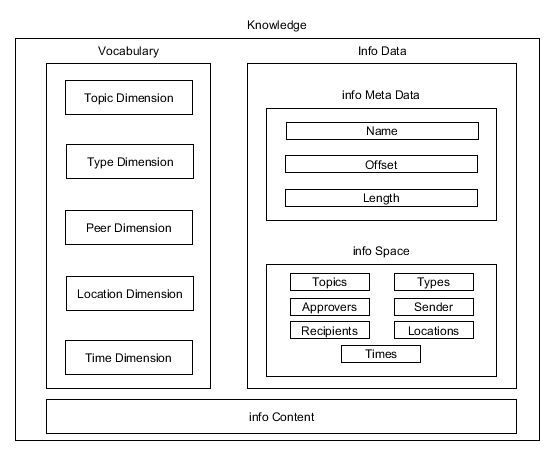
\includegraphics[width=0.9\linewidth]{general/Knowledge.png}}%
	\caption{Die ASIP/Shark Bestandtteile im Überblick}
	\label{fig:knowledge}
\end{figure}
Die beiden wichtigsten Kommandos des Protokolls sind:
\begin{itemize}
	\item Insert: Dieser Befehl wird dazu benutzt, um neue Informationen (bzw. Wissen) von anderen Peers der eigenen Wissensbasis hinzuzufügen. Dieses Wissen ist folgendermaßen unterteilt:
	\begin{itemize}
		\item Das Vokabular des Peers welches alle ihm bekannten Wörter enthält. Die Wörter sind wiederum in die fünf Dimensionen Topic, Type, Peer, Location und Time unterteilt.
		\item Der eigentliche Informationsinhalt in Form eines byte Streams mit Rohdaten.
		\item Technische Metadaten über den Informationsinhalt wie beispielsweise die Anzahl der Bytes
		\item Semantische Metadaten über den Informationsinhalt in Form der in Tabelle x.x beschriebenen sieben Dimensionen, technisch umgesetzt mit Behältern von \textit{Semantic Tags}.		
	\end{itemize} 
	\item Expose: Neben dem Hinzufügen von neuen Wissen haben Peers auch die Möglichkeit, ihr Interesse an neuem Wissen gegenüber anderen Peers zu bekunden. Dies geschieht über den Befehl \textit{Expose}, wobei auch hier das Interesse in Form der in Tabelle x.x dargestellten sieben Dimensionen formuliert wird.
\end{itemize}
[...]

\subsubsection{SharkNet}

SharkNet ist ein dezentrales soziales Netzwerk für Android Geräte und wurde von Michael Schwarz und Prof. Dr.-Ing. Thomas Schwotzer von 2015 bis 2017 entwickelt. Es kann durch die folgenden drei Kernaspekte beschrieben werden:
\begin{itemize}
	\item Dezentraler Datenaustausch ohne der Verwendung eines Servers
	\item Eine Public-Key-Infrastruktur, womit die Kommunikationspartner sich gegenseitig authentifizieren können
	\item Ausschließliche Benutzung von Open-Source Bilbiotheken und Protokollen
\end{itemize}
SharkNet bildet die Grundlage für diese Arbeit und wurde an diversen Stellen weiterentwickelt, wobei auch einige Probleme im Bereich der Kommunikation zwischen den Peers behoben werden mussten. Die ursprüngliche Zielgruppe von SharkNet sind Schüler der Katholischen Theresienschule Berlin, die als Testpersonen SharkNet anstelle von Facebook oder anderen servergebundenen sozialen Netzwerken nutzen sollten. Über die Webseite \url{http://sharedknowledge.github.io/} kann bereits ein Prototyp heruntergeladen werden, dieser enthält aber noch nicht die eigentliche Kernfunktionalität, daher keinen Chat bzw. Gruppenchat. Ein wichtiger Bestandteil dieser Arbeit ist es daher, neben dem semantischen Broadcast auch die normale Chatfunktionalität für den Endanwender benutzbar zu machen.  
\newline[...]
\newpage



